\documentclass[conference]{IEEEtran}
\IEEEoverridecommandlockouts
% The preceding line is only needed to identify funding in the first footnote. If that is unneeded, please comment it out.
\usepackage{kotex}
\usepackage{cite}
\usepackage{amsmath,amssymb,amsfonts}
\usepackage{algorithmic}
\usepackage{graphicx}
\usepackage{textcomp}
\usepackage{xcolor}
\usepackage{cleveref, array, booktabs, threeparttable}
\usepackage{array}
\usepackage{tabu} 
\usepackage{enumitem}
\usepackage[export]{adjustbox}
\def\BibTeX{{\rm B\kern-.05em{\sc i\kern-.025em b}\kern-.08em
    T\kern-.1667em\lower.7ex\hbox{E}\kern-.125emX}}
\begin{document}

\title{보름달 – Period Tracker with NUGU Speaker\\
{\footnotesize \textsuperscript{*}Team Name : Passengers}
}

\author{\IEEEauthorblockN{Jegou du Laz Theophile}
\IEEEauthorblockA{\textit{dept. Electrical Engineering,} \\
\textit{ESILV Univ.}\\
Paris, France \\
theophile.dulaz@gmail.com }
\and
\IEEEauthorblockN{Jung Sihyun}
\IEEEauthorblockA{\textit{dept. Information System,} \\
\textit{Hanyang Univ.}\\
Seoul, Republic of Korea  \\
tlgus0226@hanyang.ac.kr}
\and
\IEEEauthorblockN{Kim Jeongin}
\IEEEauthorblockA{\textit{dept. Information System,} \\
\textit{Hanyang Univ.}\\
Seoul, Republic of Korea \\
kji990607@gmail.com}
\and
\IEEEauthorblockN{Kim Jina}
\IEEEauthorblockA{\textit{dept. Information System,} \\
\textit{Hanyang Univ.}\\
Seoul, Republic of Korea \\
wlsdk7245@naver.com}
}

\maketitle

\begin{abstract}
In modern society, because of various social problems, many women suffer from ovary disease, premature menopause, and infertility. The number of women with menstrual disorders has increased compared to the past. For woman’s health, the establishment of menstrual cycle is greatly important. Although there are so many functions in NUGU speaker, there is no service about period tracker. That’s why we decided to develop this service, ‘보름달.’ It can be very good helper for woman not only in terms of technical functions, but also emotional functions.
\end{abstract}

\begin{IEEEkeywords}
menstrual cycle, period tracker application, NUGU speaker, Full-moon, and etc.
\end{IEEEkeywords}

\begin{table}[ht!] \renewcommand\arraystretch{1.25}
  \begin{threeparttable}
      \caption{Role Assignments(till the middle of the term)%
      \label{tab:table1}}    %% Caption above tabular, label inside caption
      \begin{tabular}{@{}l l>{\raggedright\arraybackslash}p{3.8cm}@{}}
      \toprule
      \bfseries Role & \bfseries Name & \multicolumn{1}{l}{\bfseries Task description and etc.} \\
      \midrule
      User & Kim Jeongin & Think of ideas and specify people's need. Design functions for our service. Also test the result in the user's perspective and give feedback. \\
      Customer & Theophile & Tries to anticipate the needs of the users to raise their interest in the product. Also works with the Developer Team to make sure that the prototypes and final product meet those requirements as much as possible. \\
      Software developer & Jung Sihyun & In charge of software development. Writes codes and make sure it executes. If problem occurs in software, settles down and develop the software. \\
      Development manager & Kim Jina & Schedules and delegates tasks required to successfully complete project's initiatives. Leads to achieve the local planning vision \& objectives. Assigns each member of the team to their own tasks. \\
      \bottomrule
      \end{tabular}
  \end{threeparttable}
\end{table}

\section{Introduction}
\subsection{Motivation}
In recent times, social situations such as extreme diet, stress, exposure to environmental hormones, and mixed nights-days threaten women uterine health. Many people suffer from polycystic ovarian syndrome, premature menopause, and infertility. The number of women with menstrual disorders has increased 3.56 times from 2000 to 2010\cite{b1}. The establishment of menstrual cycles is important, not just for fertility or convenience of preparing for the next period, but also because it is a basic index of women's health. Thus, period tracker applications are essential for women. 

However, service related to menstruation is not provided in NUGU speakers currently. If this service is available with a voice-based system, the small change will lead to certain convenience in women's daily lives.

Meanwhile, most women go through uncontrollable mood swings and pain as a part of PMS (premenstrual syndrome). Though NUGU speakers are not real people, they can be comforting to users, referring to SKT. They analyzed NUGU speakers and reported that the word "I love you" is spoken the most by users. Users want emotional interaction with AI speakers. Therefore, we planned a service, 보름달 which can satisfy the technical and also the emotional aspects at the same time, so that it can be helpful to women who are having a hard time because of PMS. 

We named our service “보름달” because the moon and women's menstruation cycle were found to be somewhat related. The moon's brightness directly affects the secretion of melatonin hormones which regulate women's menstrual cycles. On a dark day when the crescent moon rises, the secretion of melatonin induces ovulation, and under the bright full moon, its secretion decreases and menstruation begins. By comparing the data of the menstrual cycle of 8,000 women around the world with changes in the moon's status, it has been confirmed that alike in the past, modern women often ovulate in the crescent and begin menstrual periods in the full moon\cite{b2}. Moreover, the monthly cycle of inner lining of the uterus to thicken and collapse is similar to that of the moon waxes and wanes.
\subsection{Problem Statement}
You run out of sanitary pads when the monthly period is upon. Menstruation begins suddenly when you are outside, so you should buy new pads at a high price though you already have plenty at home. They are all common situations to women in childbearing age, but it's still embarrassing. That’s the reason many women use period tracking mobile applications which send notifications. However, there is a problem. 

You may have seen a lot of notifications on the mobile phone when you wake up in the morning. Morning alarm, missed calls overnight, push notifications from various applications, etc. You may usually ignore those alerts, because many people choose to erase them all rather than checking one by one. If you choose to receive alerts, it's uncomfortable to see unnecessary information. On the contrary, if you choose not to receive notifications, you can't get any useful information at all. 보름달 service based on NUGU speakers will send the notifications only what you want.

When you use mobile applications, you have to go through a series of steps to find where the cell phone is, unlock it, enter the app and find the information you want. Although you are accustomed to it, these steps may bother you. With NUGU Speakers, a tiresome process is not needed. All you have to do is just to call NUGU and ask for information. On a busy morning, you can get the information you need quickly and accurately with a short conversation instead of the hassle of checking the application.

보름달 automatically calculates and records menstrual cycles, and you can also manage physical condition by entering a BMI index. NUGU asks you whether to order relevant products like sanitary pads, ovulation tester, or pregnancy tester, affiliating with ‘11st’ when the period approaches. It is also possible to record physical symptoms to help and detect diseases which initial treatment is important, such as venereal disease and vaginitis. In addition, NUGU lets you know information on birth control pills and alerts you not to miss time since the pills must be taken at the same time everyday. 

This is not all of our service. 보름달 will be a good friend when you plan to have children. It will take care of your sex life by checking your sexuality and possibility of pregnancy. It will provide exercise information, food information, and tips in accordance with your menstruation cycle.

\subsection{Research on Related Software}
Multiple applications with similar features are already available on the App store and the Play store (Apple and Android).

Here are a few examples: 

The first one is “Period Tracker”. It’s the most downloaded menstrual period tracker app on the Play store with more than 100M downloads. It allows you to monitor your menstrual cycle and ovulation cycle. With this app you can follow your chances of being pregnant or get pregnant daily. It also monitors your sexual life, weight, body temperature, symptoms and mood. Based on this information it allows you to keep an eye on your menstrual cycle as well as to lose weight while staying healthy at all time. Furthermore, the app notifies you when your periods might start and when to take the pill. Your data is saved on a database and linked to your google Account, so you don’t lose anything even when changing the device you’re using it with. How does it work: you Get a daily check of symptoms, mood, water drinking … to determine your health and better monitor your menstrual cycle. Based on your personal history (that you can access on the app) and your previous daily check, you get previsions on your next menstrual cycle, fertility and time to take the pill for example. 

Another example is “Flo” (50M+ downloads on the Play store), a very similar app with added features. Indeed, it has all the features offered by the previous app and plus, it offers mental and physical health related features. For example, the app can suggest physical training based on your physical health and suggest stories to help you go to bed and/or help you get rid of anxiety. This app monitors more things to be able to suggest physical training. It monitors your sleep and number of steps to be able to provide this feature for instance. The App also provides advice to take care of a baby, thus accompanying you even after pregnancy.

One thing to notice though, is that none of the most popular and used applications provide voice recognition features such as what 보름달 wants to achieve, thus giving us more reasons to develop such a service. Right now, to be able to use such a service, you have to carry your phone and be aware of notifications even at home where it should be a  relaxing place. Being able to speak in a natural conversation with an AI on such a sensitive and personal subject is not a thing yet.

\section{REQUIREMENTS}

\subsection{Functional Requirements}
\begin{itemize}
\setlength{\parindent}{2ex}
\item NUGU Speaker

NUGU speaker processes instructions received from the mobile application, and voice instructions.
\begin{enumerate}
\item NUGU spekaer starts 보름달 application.
\item NUGU speaker records the user’s menstrual start and end dates by recognizing voice.

ex) I started my period.
\item NUGU speaker records dates that the user had sex by recognizing voice.

ex) I made love. 
\item NUGU speaker records the user's physical condition, mood, weight and height by recognizing voice.

ex) I weigh -kg today.
\item NUGU speaker informs the expected date and period. 
\item NUGU speaker asks whether to order sanitary pads in connection with  "11st" when the scheduled date is imminent.

ex) Your next period is in 5 days. Do you want to order sanitary pads on '11st'?
\item Nugu speaker informs the possibility of pregnancy based on the entered data of the day of sexual relation.

ex) The possibility of prestige today is -\%. If you are on birth control, be careful!
\item NUGU speaker alerts you when to take contraceptives. It also tells you how to take it according to the user's request.
ex) It's 11 a.m. time for contraceptives.

\item NUGU speaker sends the user's requests to mobile application.
\item NUGU speaker answers the user’s questions based on stored data.

ex) When will my next period start? - It will be in 6 days.
\item NUGU speaker tells users how to relieve PMS.
\item NUGU speaker says comforting words.

ex) You are not alone. Don’t be lonely.
\end{enumerate}
\end{itemize}

\begin{itemize}
\setlength{\parindent}{2ex}
\item Mobile Application

보름달 is an IOS and Android application. In the full moon application, the user can use all of the functions available on NUGU speaker. (Voice-based alerts will be replaced by push notifications.) The full moon application allows the users to check out and enter further information visually.
\begin{enumerate}
\item The full moon is an IOS and Android application.
\item The application calculates menstrual cycle and shows due date on the calendar. 
\item The application informs the users how to take, where to buy contraceptives. It sends push alerts to take pills.
\item The application affiliates with ‘11st’ to buy ovulation and pregnancy testers.
\item The application analyzes entered symptoms and checks various diseases such as STD and vaginitis.
\item The application calculates the possibility of pregnancy by setting pregnancy mode.
\item The application provides exercise, food, daily life tips on menstruation to help users.
\end{enumerate}
\end{itemize}


\subsection{Non-Functional Requirements}
\begin{itemize}
\item User Management
\begin{enumerate}
\item Download an app (Both available in IOS and Android)
\item Create a user account
\item Enter the user’s menstrual information.
If the user doesn’t remember, start to make a record from the first month.
\item Record information
Information that the user entered through NUGU speaker and the application will be stored in the database.
\item Automatic calculation
Calculates menstrual cycles and ovulation dates based on the user’s information entered.
\item Register the payment method on the ‘11st’ application.
For automatic ordering, the first agreement on the terms and conditions is also necessary.
\item Informs the user of her menstruation cycle.
\end{enumerate}
\end{itemize}

\section{DEVELOPMENT ENVIRONMENT}
\subsection{Choice of software development platform}
\begin{itemize}
\setlength{\parindent}{2ex}
    \item Development Platform
    \begin{enumerate}
    \setlength{\parindent}{2ex}
        \item Windows10  
        
        We use Windows10. Microsoft's Windows is the most common platform in the world, accounting for 77.74\% of all computer platforms as of 2020, and Windows10 accounts for 74\%.\cite{b3}
        \item Android 
        
        We make an application which works with NUGU speaker. Our application is available on Android, which accounts for 74.43\% of all mobile platforms.\cite{b4}
        
        \item iOS  
        
        Our 보름달 service is also available in iOS, which accounts the quarter of all mobile operating system platforms.\cite{b5}
    \end{enumerate}
\end{itemize}
\vspace{0.5mm}

\begin{itemize}
    \item Programming Language
    \begin{enumerate}
    \setlength{\parindent}{2ex}
    \item Javascript
    
    Javascript is an object-based script language mainly used for web browsers along with HTML and CSS. HTML adds meaning to raw content by marking it up, CSS formats the marked up content, and finally javascript makes the content and formatting interactive.
    
    It is high-level, multi-paradigm and supports event-driven, functional, and imperative programming styles. Despite original purpose to make web browsers, it is now possible to build servers. Javascript is also platform independent. These are the main reasons we choose JavaScript. Specifically, we use React as a frontend and Node.js as a backend.
    \item python
    
    Python is an interpreted, object-oriented, high-level programming language. Python supports modules and packages. Its interpreter and the extensive standard library are available in source or binary form without charge for all major platforms, and can be freely distributed.
    
    We use python tensorflow for machine learning.

    \end{enumerate}
\end{itemize}
\vspace{0.5mm}
\begin{itemize}

    \item Development Environment 
    \begin{enumerate}
    \setlength{\parindent}{2ex}
        \item Visual studio code
        
        Visual studio code is Microsoft's source-code editor which includes the Javascript by default.
        \item Webstorm
        
        Webstorm is an IDE for modern JavaScript development equipped for complex client-side development and server-side development with Node.js.
        \item Git \& Github
        
        Git and github provide three main functions. The first is version control. Git is a version control system to store when and what changes have been made to a file. The second is back-up. If the data is stored only on a local computer, it will eventually be lost, so it needs to be saved. GitHub is the remote storage of the Git, which provides online backup. Lastly, github provides a powerful function of collaboration. When people work as a team, they can push and pull their source codes to remote storage to work together. 
        
        We use them to manage our source code. 
        \item Overleaf
        
        Overleaf is an online collaborative writing and publishing tool that makes the whole process of writing, editing and publishing scientific documents much quicker and easier. Overleaf provides the convenience of an easy-to-use LaTeX editor with real-time collaboration and the fully compiled output produced automatically in the background as you type. 
        
        We use overleaf to collaborate in real time.\cite{b7} 
        \item NUGU playbuilder
        
        NUGU playbuilder connects to NUGU speakers and supports a variety of services of NUGU, SK telecom’s artificial intelligence speaker. NUGU platform first identifies the intention of user utterance through voice recognition and natural language understanding. Then, it properly acts and responds through text-to-speech. Nugu playbuilder is a GUI based integrated development environment that offers techniques needed in this process.  
        \item Adobe XD
        
        Adobe XD is an all-in-one UX/UI solution to design websites, mobile apps and more.
        
        We use this to make prototype for our service and share with team members. We referred to the prototype in the development process.
        \item Slack
        
        Slack is a channel-based messaging platform and cloud-based collaborative web application.
        
        We use slack to communicate. We can work together more effectively, as connected to all software tools and services like github, trello, google spreadsheets.
        \item Visual Paradigm
        
        Visual Paradigm is a UML diagram drawing tool that helps us intuitively grasp the structure.
        
        We use Visual Paradigm to draw diagrams.
        \item Node.js (Backend)
        
        Node.js is a single thread non-blocking model which is relatively easy to learn for people who are not familiar with server programs. The advantages of being able to develop websites in one language of JavaScript leads to high productivity and is compatible with json format. However, it is not suitable for servers that use CPU a lot, such as large-scale images or video processing. 
        
        We judged that our service does not use much CPU, and the advantage would be a lot bigger. So we use node.js as backend.
        \item MySQL (Database)
        
        SQL is a stable and consistent form of database. Among them, MySQL is the most popular open source Relational SQL Database Management System. MySQL is one of the best RDBMS being used for developing various web-based software applications.
        
        We chose SQL rather than NoSQL because of the characteristics of our database. It has sets of related and structured tables like users, cycles, and pills.
        \item React (Frontend)
        
        React is a library that provides only ‘view’ among MVC patterns and can be implemented using JavaScript. When certain elements change, they can render only the necessary parts through DOM monitoring rather than re-rendering the whole. So it reduces unnecessary resource consumption and improves Web app performance.
        
        We choose react for frontend development to provide a comfortable user experience while saving the most performance as possible.
        \item Amazon EC2
        
        Amazon Elastic Compute Cloud (Amazon EC2) provides scalable computing capacity in the Amazon Web Services (AWS) Cloud. Using Amazon EC2 eliminates user’s need to invest in hardware up front, so we can develop and deploy applications faster. \cite{b8}
        \item Tensorflow
        
        TensorFlow is an open-source library which is popular with Machine Learning. TensorFlow offers APIs that facilitates Machine Learning.
        The goal is to implement this AI model in using NUGU speaker.
    \end{enumerate}
\end{itemize}

\begin{itemize}
    \item Cost Estimation
\begin{table}[h]
\centering
\caption{Cost Estimation}
\begin{tabular}[t]{p{0.8cm}p{3.4cm}p{2.5cm}}
\toprule
Type&Content&Price\\
\midrule
Labor&4 People * 10,308won * 200 hours&8,246,400 won\\
\rule{0in}{3ex}Laptop&LG AllDayGram i3 7th Gen&1,860,000 won\\
\rule{0in}{2ex}&Samsung PenS i5 8th Gen&2,030,000 won * 2\\
\rule{0in}{2ex}&Xiaomi Mi Notebook Pro i5&1,010,000 won\\
\rule{0in}{3ex}Internet&SK broadband internet&16,500won per month\\
\rule{0in}{3ex}Program&Overleaf&8 dollars per month\\
\rule{0in}{3ex}Venue&&\\
\bottomrule
\end{tabular}
\end{table}%

\end{itemize}
\subsection{Software in Use}
\begin{itemize}
    \setlength{\parindent}{2ex}
    \item Existing Period-Tracker Applications (ex. Flo, Bom Calendar, Pink Diary etc.): These applications inform menstruation cycles and deliver various notifications through push alarms. However, reckless push alarms prevent users from picking up the necessary information, and excessive advertising within the applications makes user uncomfortable.
    
    We use Nugu speaker to get the information only we want quickly through voice-based service, and we will not add advertisements to seek user convenience.
\end{itemize}

\subsection{Task Distribution}
\begin{table}[h]
\centering
\caption{Task distribution}
\begin{tabular}[t]{ll}
\toprule
Name&Task Description\\
\midrule
Kim Jeongin&Backend, Nugu Playbuilder\\
Kim Jina&Frontend, Nugu Playbuilder\\
Jung Sihyun&Backend, Nugu Playbuilder\\
Jwdou du Las Theophile&Machine Learning\\
\bottomrule
\end{tabular}
\end{table}%



\section{SPECIFICATIONS}
\subsection{Mobile Application}
\begin{itemize}
\setlength{\parindent}{2ex}
    \item Application Icon
    \begin{figure}[htbp]
    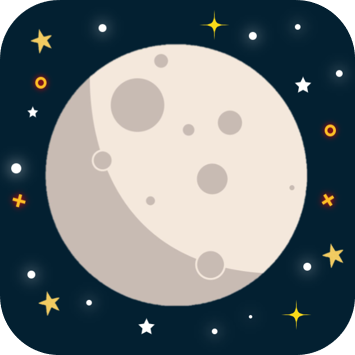
\includegraphics[width=2cm, height=2cm, center]{icon.png}
    \caption{Application Icon}
    \label{fig : Icon}
    \end{figure}
    
    \item Entry Page
    \begin{figure}[htbp]
    
\includegraphics[width=4cm, height=8cm, center]{EntryPage.png}
    \caption{Entry Page}
    \label{fig : Entry Page}
    \end{figure}
    
    This is the first screen that user see when they run the application. This screen is visible for 0.5 seconds after execution and automatically redirects to Fig. 2.
    \item Login
    
    \begin{figure}[htbp]
    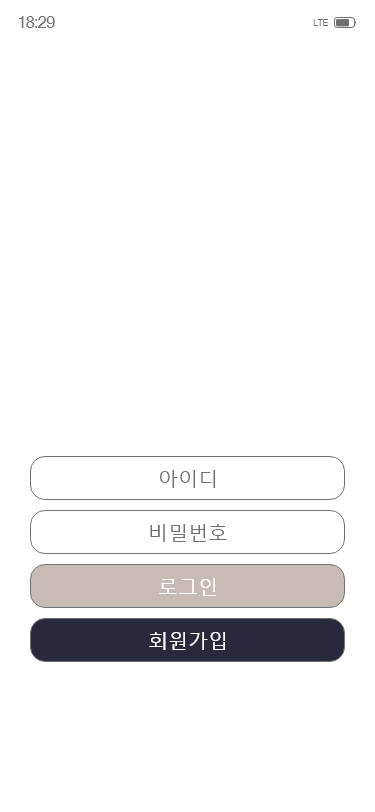
\includegraphics[width=4cm, height=8cm, center]{LogIn.png}
    \caption{Login}
    \label{fig : LogIn}
    \end{figure}
    [Fig. 3] comes after the automatically turned off [Fig. 2].  This page is for login. To register, click the register button to go to the register page [Fig. 4].  
    User enters userEmail in email format and userPassword. If there is no userEmail corresponding to the userEmail in the database, it shows ‘Wrong email’. If the userPassword is not correct, it shows ‘Wrong password’. 

    If the userEmail and userPassword are both right, the user can login and redirect to [Fig.5] main page.

    When the user forgets the password, she can use userEmail to get an email to change the password.

    \item Register
    
    \begin{figure}[htbp]
    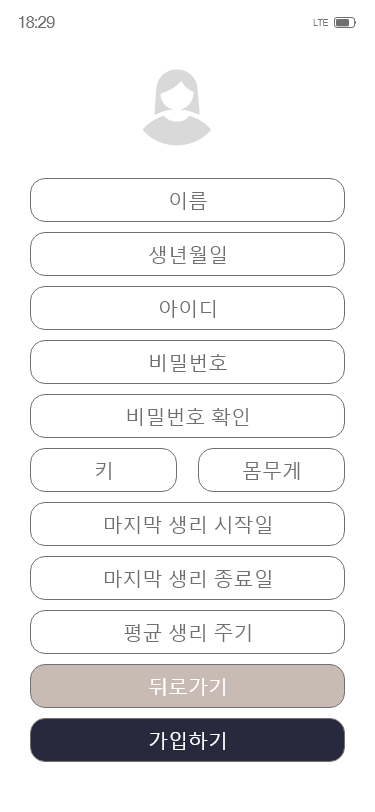
\includegraphics[width=4cm, height=8cm, center]{SignUp.png}
    \caption{Register}
    \label{fig : Register}
    \end{figure}
    User can create a new account on this page. UserName, userBirth, userEmail, userPassword and passwordConfirm are essential and UserEmail must be unique. UserHeight, userWeight, firCycleStart, firCycleEnd and meanPeriod can be optionally entered for more accurate menstrual cycle prediction. The information is stored on our database. 
    
    UserPassword and passwordConfirm must be exactly the same. UserEmail must be email format like ‘Passengers@hanyang.ac.kr’. User cannot set firCycleStart, firCycleEnd and meanPeriod as the future time compared to current time. UserHeight, userWeight and meanPeriod must be integers. UserHeight and userWeight are used to calculate BMI indices that affect menstrual cycles. 
    
    If the user clicks ‘뒤로가기(back)’ button, she can go to [Fig.3] login page. If the user clicks ‘회원가입(register)’ button, the message to congratulate success of signing up appears, and she will be redirected to [Fig.3] login page. If an error occurs, a message says that the register failed.

    \item Main Page
    \begin{figure}[htbp]
    
\includegraphics[width=4cm, height=8cm, center]{Main.png}
    \caption{Main Page}
    \label{fig : Main Page}
    \end{figure}
    
    This is the main page of our application 보름달. User information can be visually checked within the large circle.
    \begin{enumerate}
    \setlength{\parindent}{2ex}
        \item Big Circle
        
        If the due date of menstruation approaches, the remaining date will be shown, and after that, it will help the user find information such as ovulation dates easily.
        Click on the circle to open a tab with detailed data. User can check start date ,end date, medicine, or sex information. The user can also record her physical condition, mood and write a simple memo.
        \item One sentence of the Day
        
        Also 보름달 gives user simple tips related to life or menstruation and offers emotional comfort.
        \item Top/Bottom Bar
        
        In the upper left corner of every page, user can see their account information. When the user clicks logout in the upper right corner, she will be redirected to the login page. 
        
        Click the icon below to go to other pages.
    \end{enumerate}
    \item Calendar
    
    \begin{figure}[htbp]
    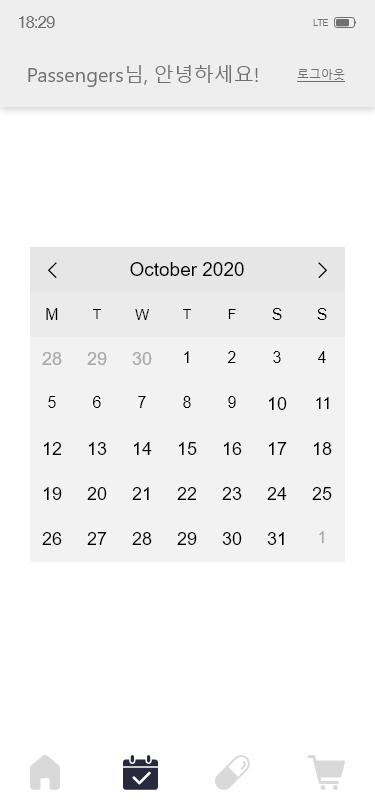
\includegraphics[width=4cm, height=8cm, center]{Calendar.png}
    \caption{Calendar}
    \label{fig : Calendar}
    \end{figure}
    
    This is a calendar page where user can view their monthly / annual calendars. Menstrual cycle and ovulation cycle can be seen at a glance on a monthly basis. User can select each date and click the date to access the calendar-detail page, Fig. 6, which was also visible on the main page.
    \begin{enumerate}
    \setlength{\parindent}{2ex}
        \item Calendar - Detail
        
        \begin{figure}[ht]
        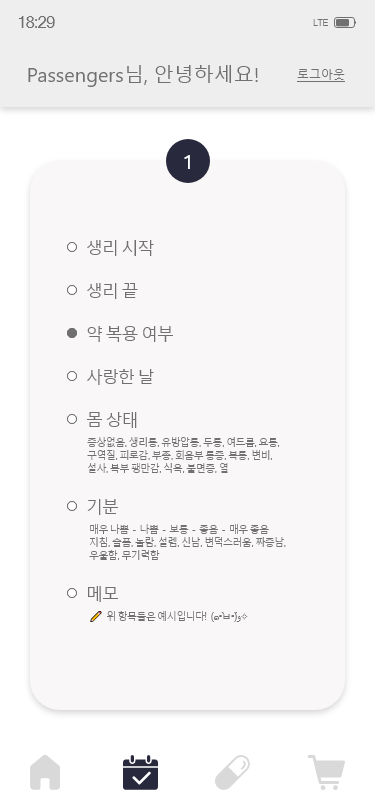
\includegraphics[width=4cm, height=8cm, center]{detail.png}
        \caption{Calendar - Detail}
        \label{fig : Detail}
        \end{figure}
        
        Even if the user doesn't set the cycle manually, the app automatically records expected days according to analyzed date. However, if there is a difference with the actual menstrual cycle, the tab's menstrual start/end check box can be used to record the exact menstrual cycle. 
        The app provides several options for body condition or mood, and the user can record in detail in the memo below.
        
        It cannot be recorded in the future based on the current date. The calendar can be seen from 1999 to 3 years later from the point. Holidays in the calendar are based on Korean holidays.

    \end{enumerate}
    \item Health 
    
    \begin{enumerate}
    \setlength{\parindent}{2ex}
        \item Pill
        
        \begin{figure}[ht]
        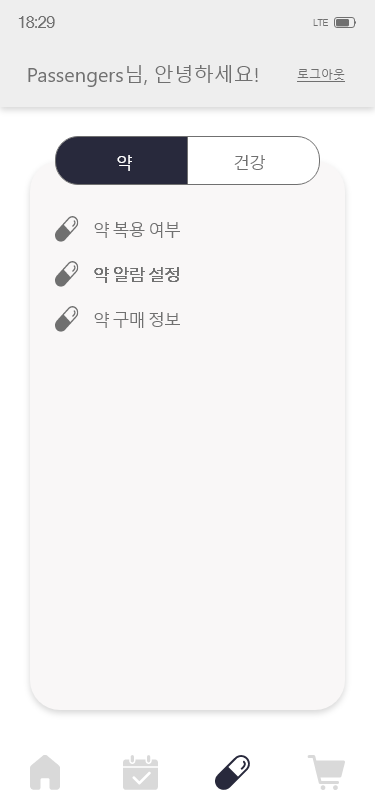
\includegraphics[width=4cm, height=8cm, center]{Health - pill.png}
        \caption{Health - Pill}
        \label{fig : Health - Pill}
        \end{figure}
        Pill tab is on the Health page. If the user sets up her own contraceptives or other medicines, the alarm rings at the same time every day until the last day of the setup to help the user take the medicine without forgetting it. 
        
        People usually take only one kind of contraceptives, so we don’t think there are many drugs that need to be taken every day by ringing the alarm, but just in case, user can register up to three drugs she’s taking in the application. If more than four registrations are desired, one of the existing drugs must be deleted.
        
        User can set a maximum period of six months for their medication. One day before the sixth month, the alarm tells the user that the alarm will be cleared the next day. And be deleted a day later.
        User can register the same pill again.

        The user can also get recommendations for contraceptives and medications for each symptom.
        \item Medi
        
        \begin{figure}[ht]
        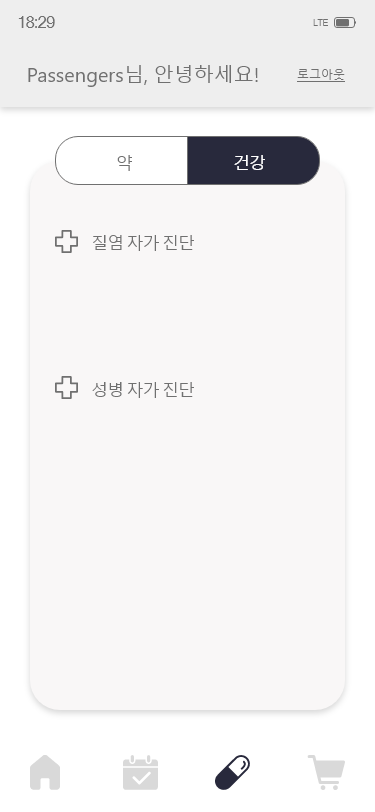
\includegraphics[width=4cm, height=8cm, center]{medi.png}
        \caption{Health - Medi}
        \label{fig : Medi}
        \end{figure}
        The user can get medical information on the medi tab on Health page.
        It provides a checklist for common venereal diseases and vaginitis. One self-diagnosis table consists of N questions that identify typical symptoms of each disease. User can keep trying self-check without restriction in a day, but the question doesn't change.

        Of course, it is most accurate to go to the hospital when suspected symptoms appear, but with this self-diagnosis card, user can check for suspected diseases faster and simpler.
    \end{enumerate}
    \item Shopping
    
    \begin{figure}[ht]
    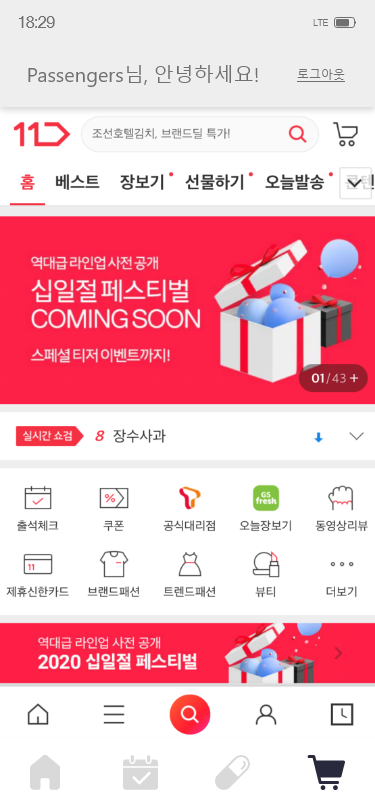
\includegraphics[width=4cm, height=8cm, center]{Shopping.png}
    \caption{Shopping}
    \label{fig : Shopping}
    \end{figure}
    
    \begin{figure}[ht]
    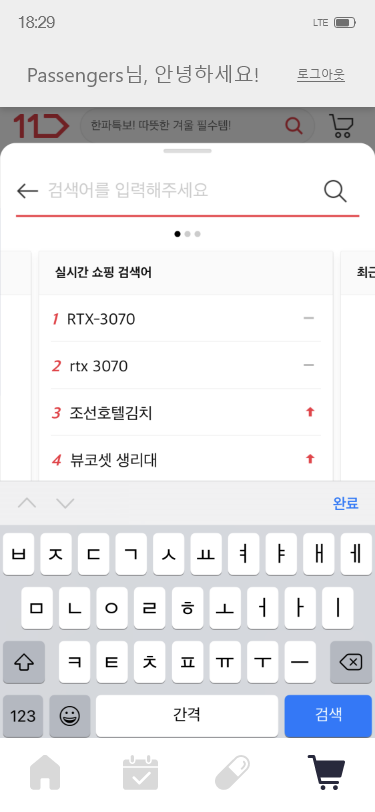
\includegraphics[width=4cm, height=8cm, center]{sh1.png}
    \caption{Shopping-1}
    \label{fig : Shopping-1}
    \end{figure}
    User can access 11st very simply within our application. User can shop easily and quickly at 11st by clicking the shopping tab at the bottom.
    They can use 11st easily as they are in the 11st application.
    
    When the menstrual due date approaches, the NUGU speaker asks you if you want to order what you need. You can also order by voice faster and simpler than the app.
\end{itemize}
\subsection{NUGU Speaker}
\begin{itemize}
\setlength{\parindent}{2ex}
    \item Action A 
    
    \begin{figure}[ht]
    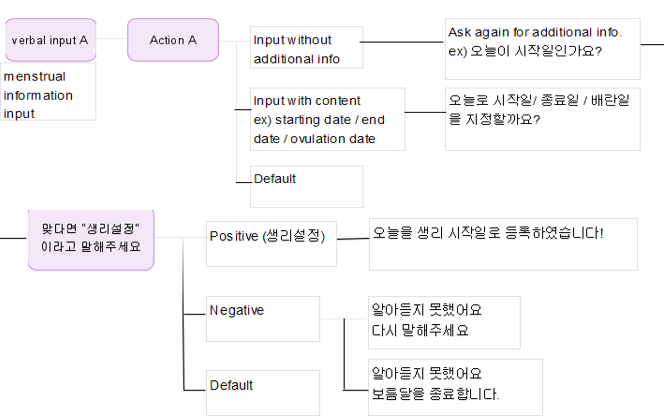
\includegraphics[width=8.5cm, height=5cm, center]{A-1.PNG}
    \caption{Action A}
    \label{fig : Action A}
    \end{figure}
    Fig. 12 shows action to enter menstrual information. Through NUGU speaker, user enters information such as the start date of menstruation, end date, ovulation date, etc., and the information is stored in our database It is used to calculate accurate menstrual cycle. \par
    
    If a user tells NUGU what kind of information it is from the first input, it can be saved through confirmation process.
    If the user does not say what kind of information it is, the speaker should ask additional questions about the type of information.
    \item Action B
    
    \begin{figure}[ht]
    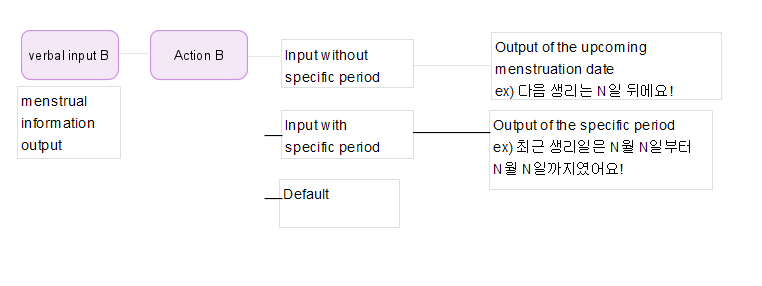
\includegraphics[width=8.5cm, height=3.8cm, right]{B.PNG}
    \caption{Action B}
    \label{fig : Action B}
    \end{figure}
    Fig. 13 is an action that outputs information related to menstrual cycles from NUGU. If a user asks a question without a specific period of time, it informs the expected date of upcoming menstruation, and if an input asks a specific period of menstruation (ex, last month, most recent), NUGU informs the menstrual date of the specific period.
    \item Action C
    
    \begin{figure}[ht]
    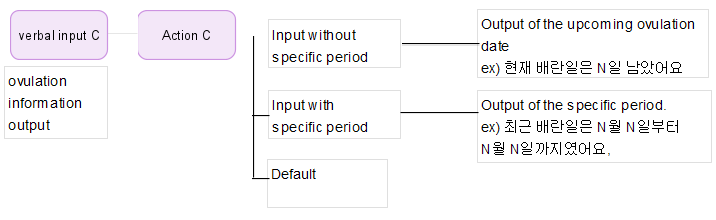
\includegraphics[width=8.5cm, height=3cm, center]{C.PNG}
    \caption{Action C}
    \label{fig : Action C}
    \end{figure}
    When a user asks about ovulation date, NUGU answers. 
    As fig.12, Action B, asking for ovulation dates for a specific period of time informs the ovulation dates for that period, or the ovulation dates that are approaching.
    \item Action D
    
    \begin{figure}[ht]
    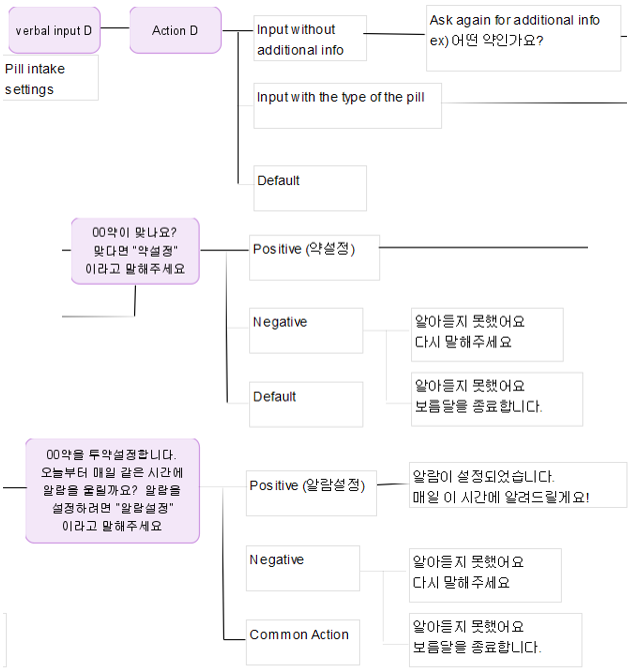
\includegraphics[width=8.5cm, height=10cm, center]{D.PNG}
    \caption{Action D}
    \label{fig : Action D}
    \end{figure}
    Fig 15. is an action that allows user to set up her own medicine-related information. If the user tells NUGU what kind of medicine it is, NUGU asks the user whether to set the alarm. If the user agrees, it rings the alarm same time every day until the last day. If the user does not set the last day, it rings daily without an end.
    When the type of drug is not mentioned in the initial input, additional question should be asked about the type of pill.
    
    \item Action E
    
    \begin{figure}[ht]
    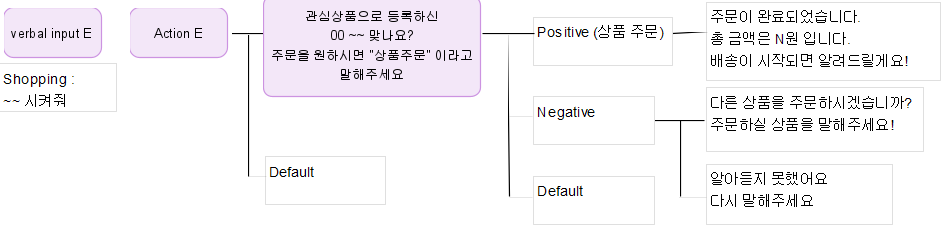
\includegraphics[width=8.5cm, height=3cm, center]{E.PNG}
    \caption{Action E}
    \label{fig : Action E}
    \end{figure}
    The NUGU speaker helps the user to shop through 11st using their voice, without turning on her internet-connected device.
    
    To place an order through voice, the user needs to log in to 11st, agree the relevant terms and conditions, register the payment method, and enter the delivery location in advance.
    T membership discount is also available if the user enters it in advance on 11st.
    It is also possible to check order details and check delivery by voice.
    
    \item Action F
    
    \begin{figure}[ht]
    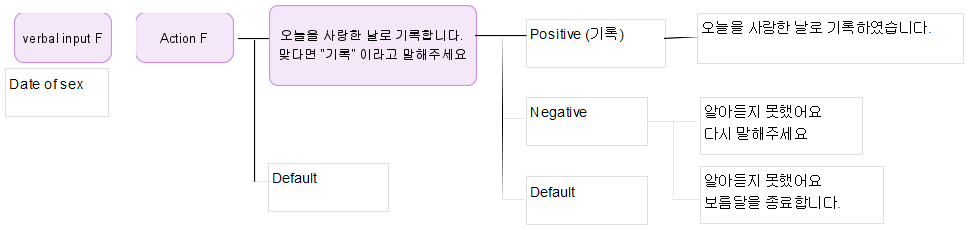
\includegraphics[width=8.5cm, height=3cm, center]{F.PNG}
    \caption{Action F}
    \label{fig : Action F}
    \end{figure}    
    Action to enter the date of sex.
    \item Action G
    
    \begin{figure}[ht]
    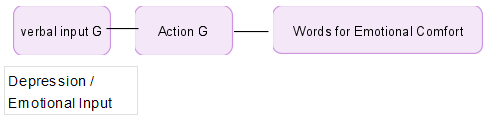
\includegraphics[width=8.5cm, height=3cm, center]{G.PNG}
    \caption{Action G}
    \label{fig : Action G}
    \end{figure}
    When the user is sad and depressed, the speaker becomes a friendly friend who gives emotional sympathy and comfort.
    
    \item Default
    
    \begin{figure}[ht]
    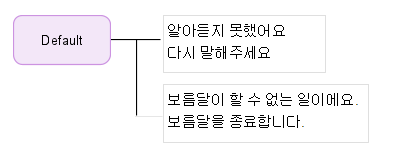
\includegraphics[width=8.5cm, height=3cm, center]{Default.PNG}
    \caption{Default}
    \label{fig : Default}
    \end{figure}
    Fig. 18 is a default ction that occurs when the speaker is unable to perform the user's demands. Default is printed when NUGU cannot understand the user's verbal input, or when NUGU is unable to execute the function.

\end{itemize}

\vspace{100cm}

\begin{thebibliography}{00}
\bibitem{b1} Korean Society of Obstetrics and Gynecology.
\bibitem{b2} Philip Chenette, a researcher at the Pacific Utility Center in the U.S. in Annual Meeting of the American Society for Biogenesis (ASRM) in Hawaii, 2014
\bibitem{b3} Statcounter – GlobalStats, Desktop Operating System Market Share Worldwide, 2020
\bibitem{b4} Statcounter – GlobalStats, Mobile Operating System Market Share Worldwide, 2020
\bibitem{b5} Statcounter – GlobalStats, Mobile Operating System Market Share Worldwide, 2020 
\bibitem{b6} 
\bibitem{b7} https://www.overleaf.com
\bibitem{b8} https://docs.aws.amazon.com/

\end{thebibliography}
\vspace{12pt}
\color{red}


\end{document}
